% Picture of the starter slide deck (scripts/gen-starters.ts compiles it to templates/starters/deck/figures/sky.pdf):
% a 300 mm x 100 mm panorama, noon on the left half, sunset on the right; the deck shows it twice, cropped
% to one half each time.
\documentclass[border=0pt]{standalone}
\usepackage{tikz}
\definecolor{noontop}{HTML}{2A64D2}\definecolor{noonlow}{HTML}{C6E2F8}
\definecolor{noonhill}{HTML}{86B98F}\definecolor{noonfront}{HTML}{4D8C62}\definecolor{cloudshade}{HTML}{D5E4F4}
\definecolor{dusktop}{HTML}{272152}\definecolor{duskmid}{HTML}{B9507A}\definecolor{dusklow}{HTML}{FFB46A}
\definecolor{duskhill}{HTML}{6B3A62}\definecolor{duskfront}{HTML}{36223F}\definecolor{dusksun}{HTML}{FFE7A8}
\definecolor{duskcloud}{HTML}{F59E70}\definecolor{duskcloudtop}{HTML}{9E4C78}
% a puffy cloud at (#1,#2), #3 times the base size, in colour #4
\newcommand\cloud[4]{\begin{scope}[shift={(#1,#2)},scale=#3]
  \fill[#4] (0,0) circle (5) (6,3) circle (6.5) (13,1.5) circle (5) (18,-0.5) circle (3.6) (-5,-1.4) circle (3.4);
  \fill[#4,rounded corners=3] (-8,-4.8) rectangle (21.5,0);\end{scope}}
\begin{document}
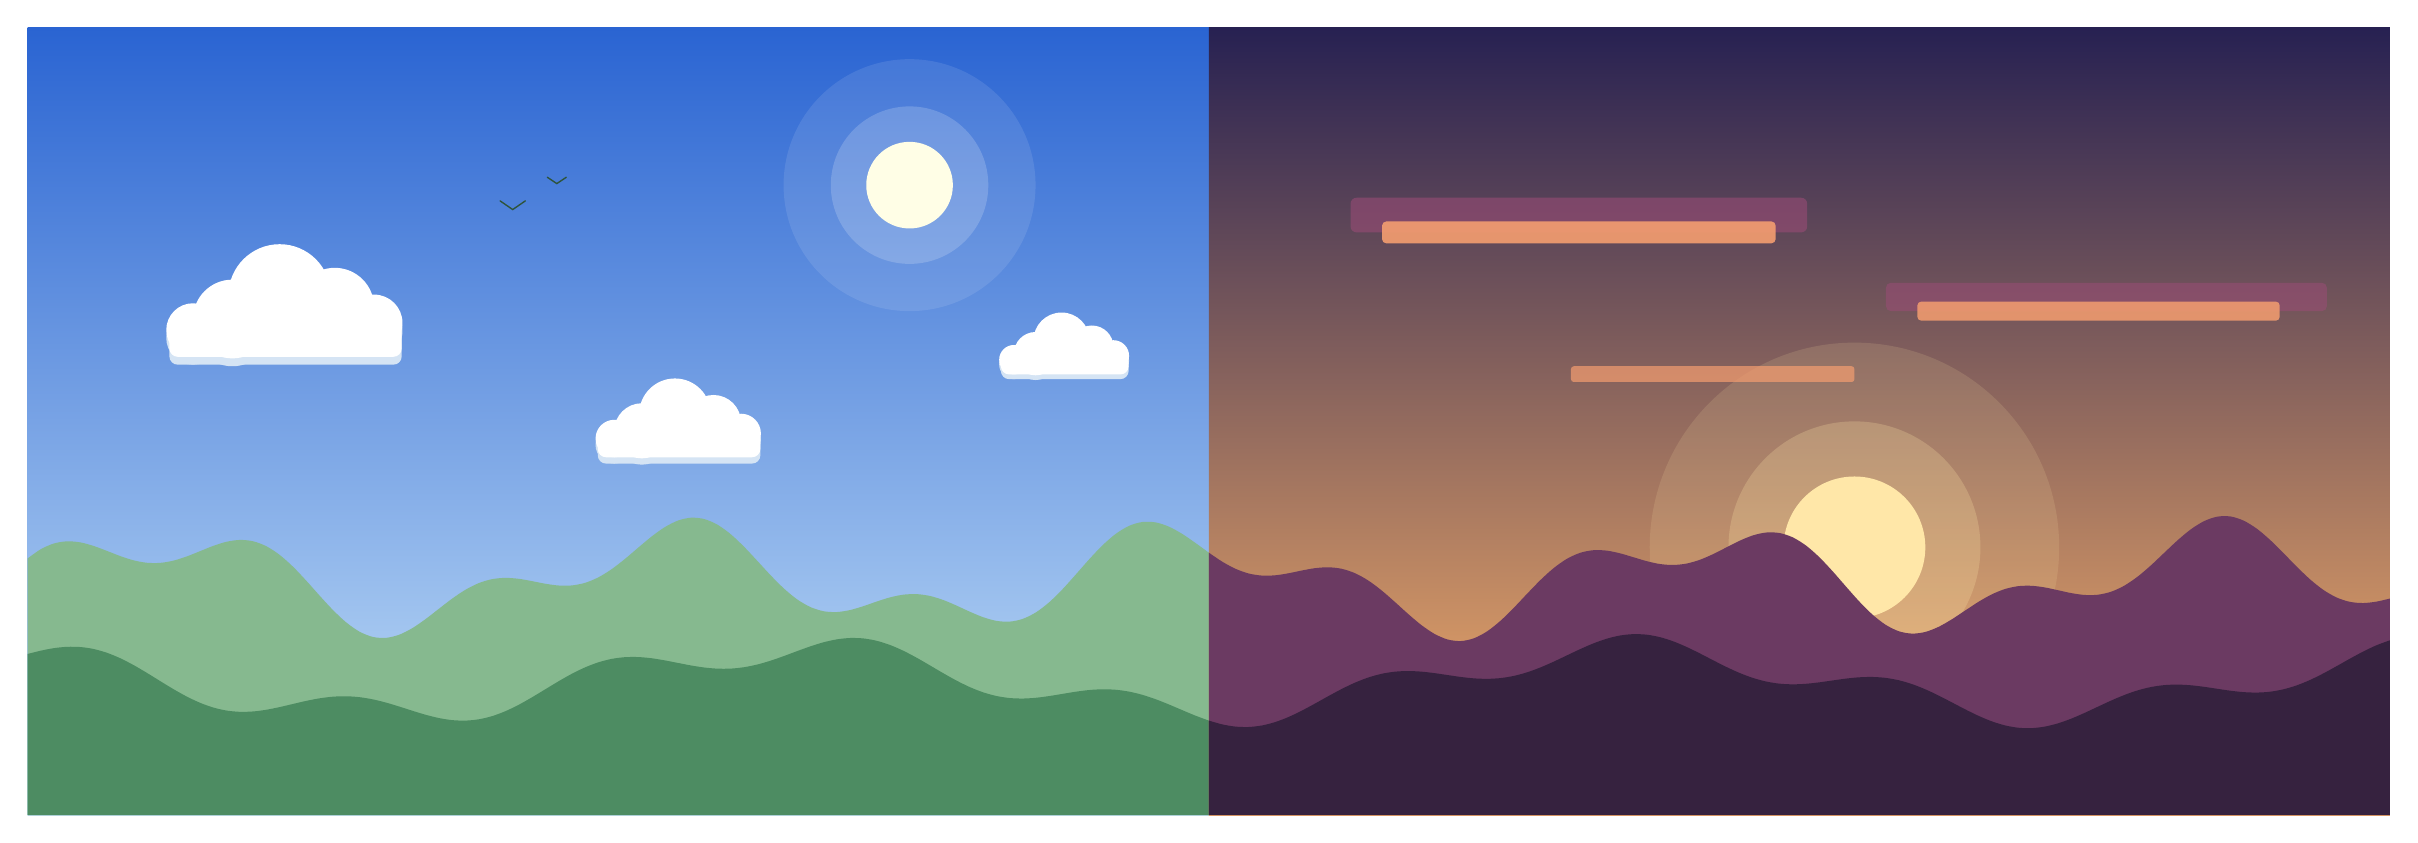
\begin{tikzpicture}[x=1mm,y=1mm]
\useasboundingbox (0,0) rectangle (300,100);
\clip (0,0) rectangle (300,100);
% noon
\shade[top color=noontop, bottom color=noonlow] (0,0) rectangle (150,100);
\fill[white, opacity=0.10] (112,80) circle (16);
\fill[white, opacity=0.18] (112,80) circle (10);
\fill[white!90!yellow] (112,80) circle (5.5);
\cloud{26}{62}{1.0}{cloudshade}\cloud{26}{63}{1.0}{white}
\cloud{78}{48}{0.7}{cloudshade}\cloud{78}{48.8}{0.7}{white}
\cloud{128}{58}{0.55}{cloudshade}\cloud{128}{58.6}{0.55}{white}
\draw[noonfront!60!black, line width=0.5, line cap=round] (60,78) -- ++(1.6,-1.1) -- ++(1.6,1.1) (66,81) -- ++(1.2,-0.8) -- ++(1.2,0.8);
\fill[noonhill] (0,0) -- plot[domain=0:150, samples=90, smooth] (\x, {30 + 5*sin(\x*5.5) + 3*sin(\x*13 + 60)}) -- (150,0) -- cycle;
\fill[noonfront] (0,0) -- plot[domain=0:150, samples=90, smooth] (\x, {17 + 4*sin(\x*3.4 + 120) + 2*sin(\x*11)}) -- (150,0) -- cycle;
% sunset
\shade[top color=dusktop, middle color=duskmid, bottom color=dusklow] (150,0) rectangle (300,100);
\fill[dusksun, opacity=0.14] (232,34) circle (26);
\fill[dusksun, opacity=0.24] (232,34) circle (16);
\fill[dusksun] (232,34) circle (9);
\fill[duskcloudtop, opacity=0.55, rounded corners=2.2] (168,74) rectangle (226,78.4);
\fill[duskcloud, opacity=0.9, rounded corners=1.6] (172,72.6) rectangle (222,75.4);
\fill[duskcloudtop, opacity=0.5, rounded corners=1.8] (236,64) rectangle (292,67.6);
\fill[duskcloud, opacity=0.85, rounded corners=1.3] (240,62.8) rectangle (286,65.2);
\fill[duskcloud, opacity=0.7, rounded corners=1] (196,55) rectangle (232,57);
\fill[duskhill] (150,0) -- plot[domain=150:300, samples=90, smooth] (\x, {30 + 5*sin(\x*5.5) + 3*sin(\x*13 + 60)}) -- (300,0) -- cycle;
\fill[duskfront] (150,0) -- plot[domain=150:300, samples=90, smooth] (\x, {17 + 4*sin(\x*3.4 + 120) + 2*sin(\x*11)}) -- (300,0) -- cycle;
\end{tikzpicture}
\end{document}
